\documentclass[../DoAn.tex]{subfiles}
\begin{document}
\section{Hệ thống quản lý rõ ràng, dễ sử dụng, minh bạch}
\subsection{Đặt vấn đề}
Hiện này nhu cầu của người tiêu dùng về việc mua và bán sản phẩm giá rẻ trên các sàn đấu giá trực tuyến ngày càng tăng cao. Đối với một website đấu giá trực tuyến thì khi dữ liệu sẽ càng ngày càng lớn, việc quản lý toàn bộ hệ thống sẽ gặp nhiều khó khăn hơn. Đặc biệt, quá trình phê duyệt các phiên đấu giá hay quản lý loại sản phẩm, thương hiệu, tin tức mất rất nhiều thời gian. Nếu Quản trị viên phải vào trong hệ thống Database để phê duyệt từng phiên đấu giá, thêm từng loại sản phẩm, thương hiệu, tin tức hay xuất dữ liệu là rất khó khăn, mất nhiều thời gian, không đảm bảo tính chính xác. Vì thế một hệ thống dành riêng cho Quản trị viên quản lý toàn bộ website là rất cần thiết. 
\subsection{Giải pháp và kết quả đạt được}
Để giải quyết vấn đề trên thì hệ thống Quản trị viên phải tối ưu hóa việc thống kê được hiện tại hệ thống đang có những gì, các trạng thái phiên đấu giá phải được chuẩn hóa chung để dễ quản lý. Hệ thống quản lý này chỉ những tài khoản có quyền Quản trị viên mới có thể đăng nhập vào và thực hiện các thao tác như phê duyệt; thêm, sửa, xóa các loại sản phẩm, thương hiệu, tin tức, slide.

Ngoài ra hệ thống cho phép Quản trị viên xuất dữ liệu ra các dạng file PDF, Excel, CSV nếu có nhu cầu in ấn thì cũng được thực hiện dễ dàng. 

Dưới đây là một số hình ảnh đến hệ thống của Quản trị viên.

Hình ảnh danh sách các phiên đấu giá hiện có trên hệ thống
\begin{figure}[H]
    \centering
    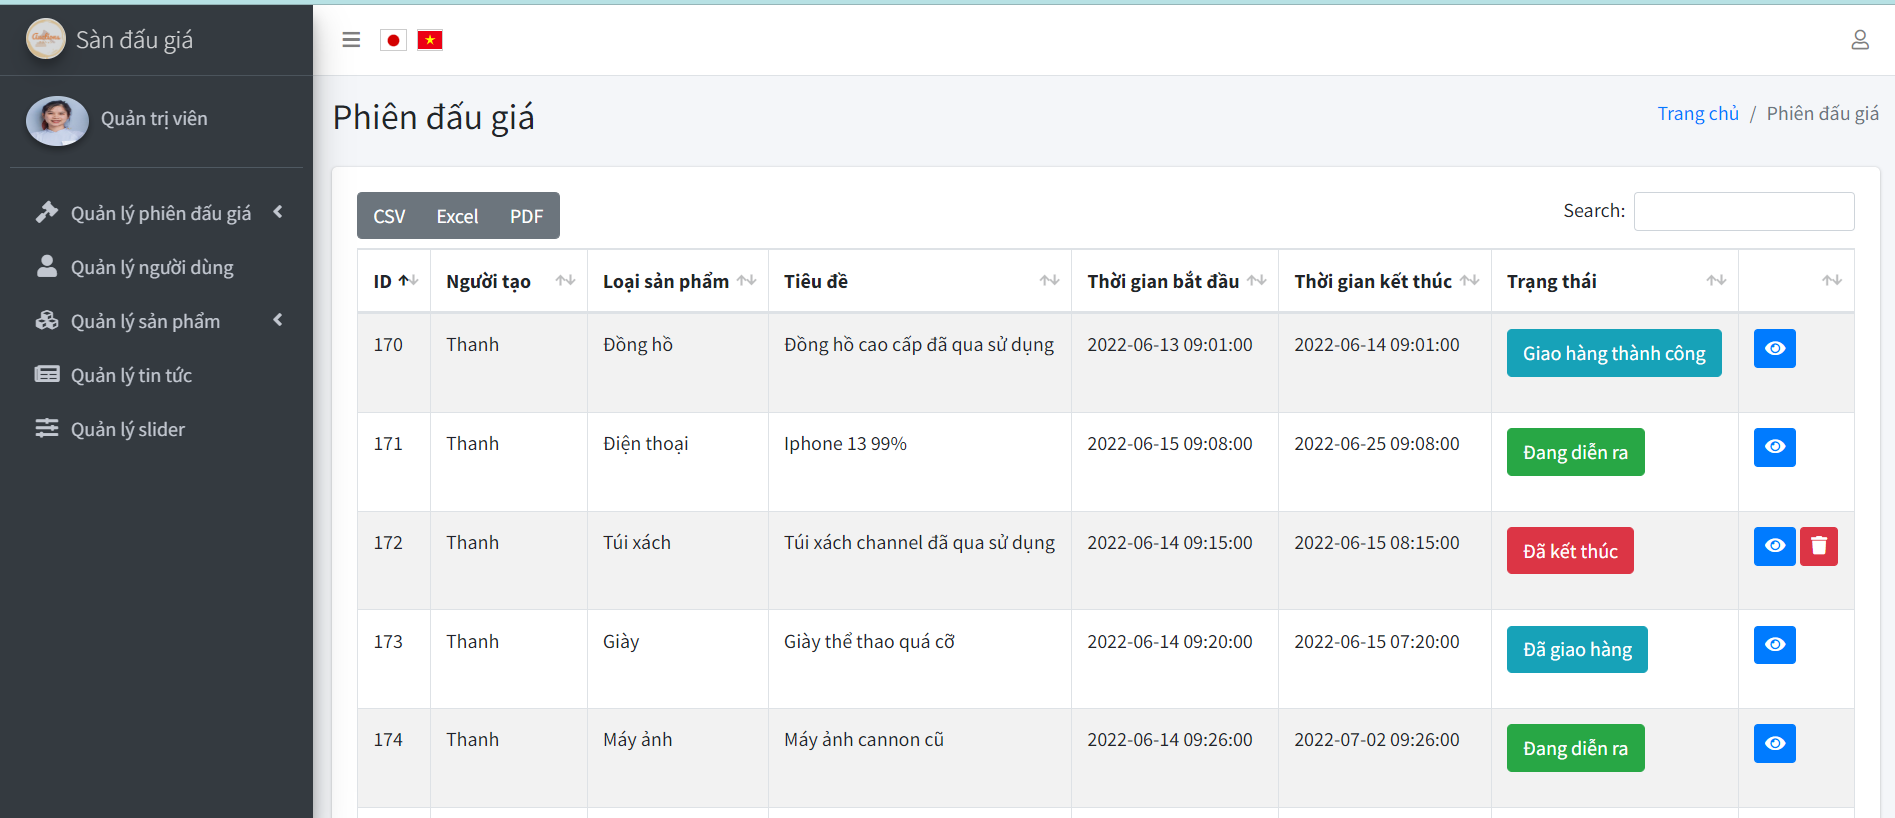
\includegraphics[width=11.4cm,height=5.0cm]{Hinhve/adminmanager.png}
\end{figure}
Quy trình đánh giá một phiên đấu giá

Quản trị viên có thể xem thông tin phiên đấu giá vừa được người dùng tạo
\begin{figure}[H]
    \centering
    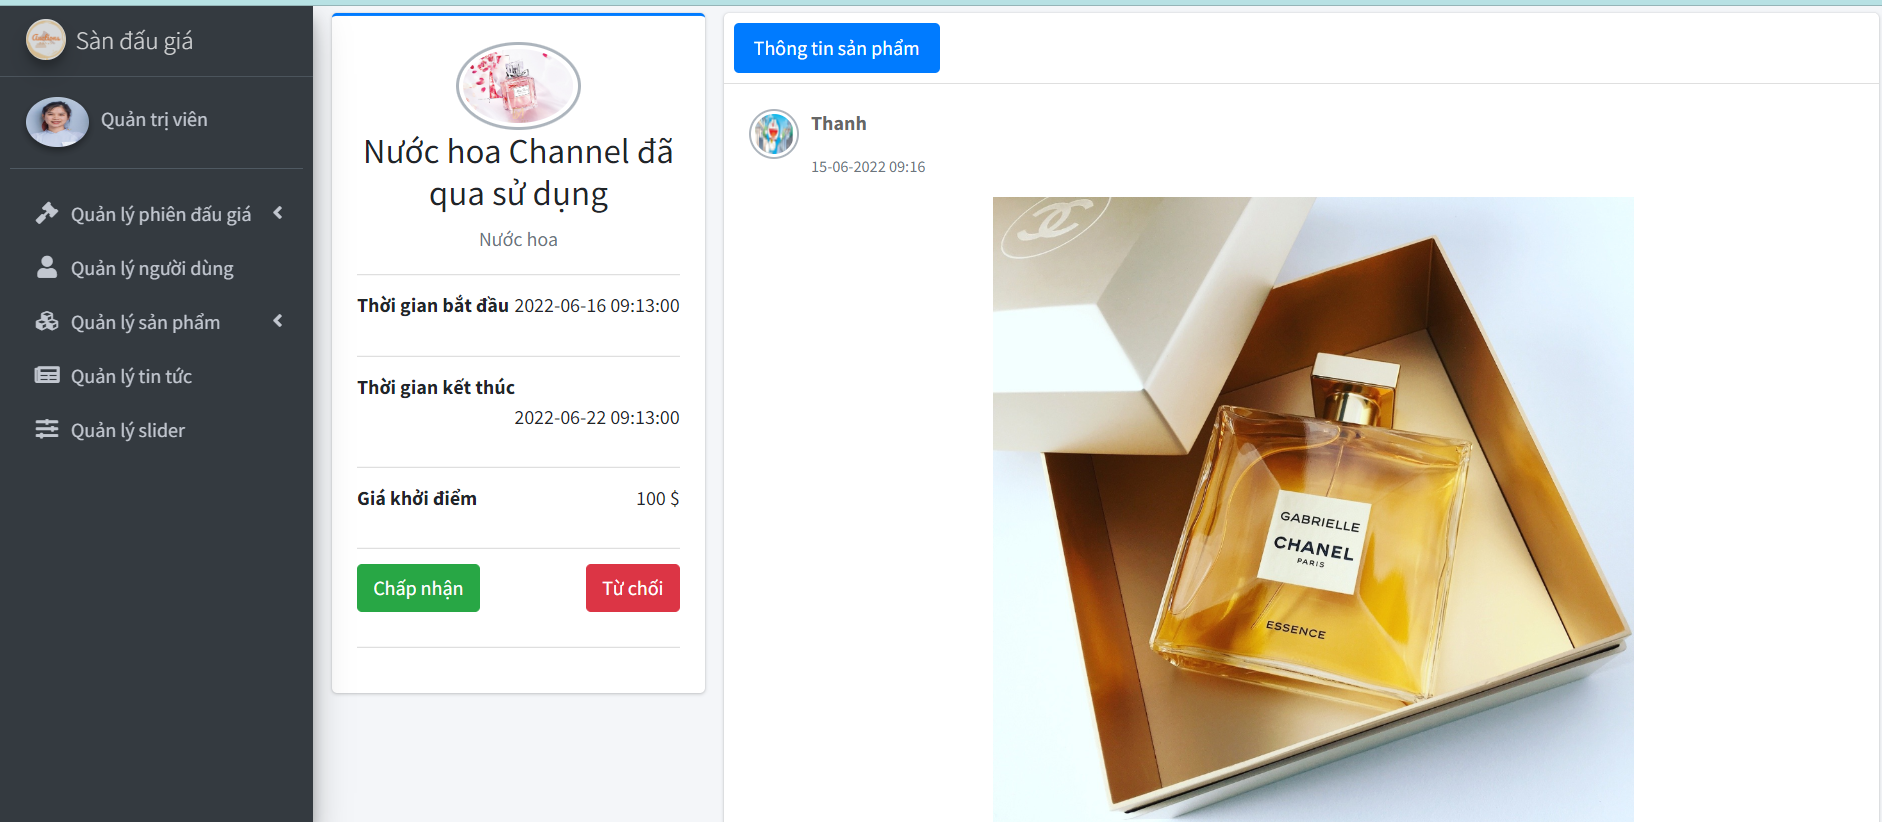
\includegraphics[width=11.4cm,height=4.96cm]{Hinhve/adminconfirm.png}
\end{figure}
Quản trị viên phải nhập đầy đủ lý do khi muốn từ chối một phiên đấu giá và hệ thống sẽ chuyển thông báo đến người tạo phiên đấu giá.
\begin{figure}[H]
    \centering
    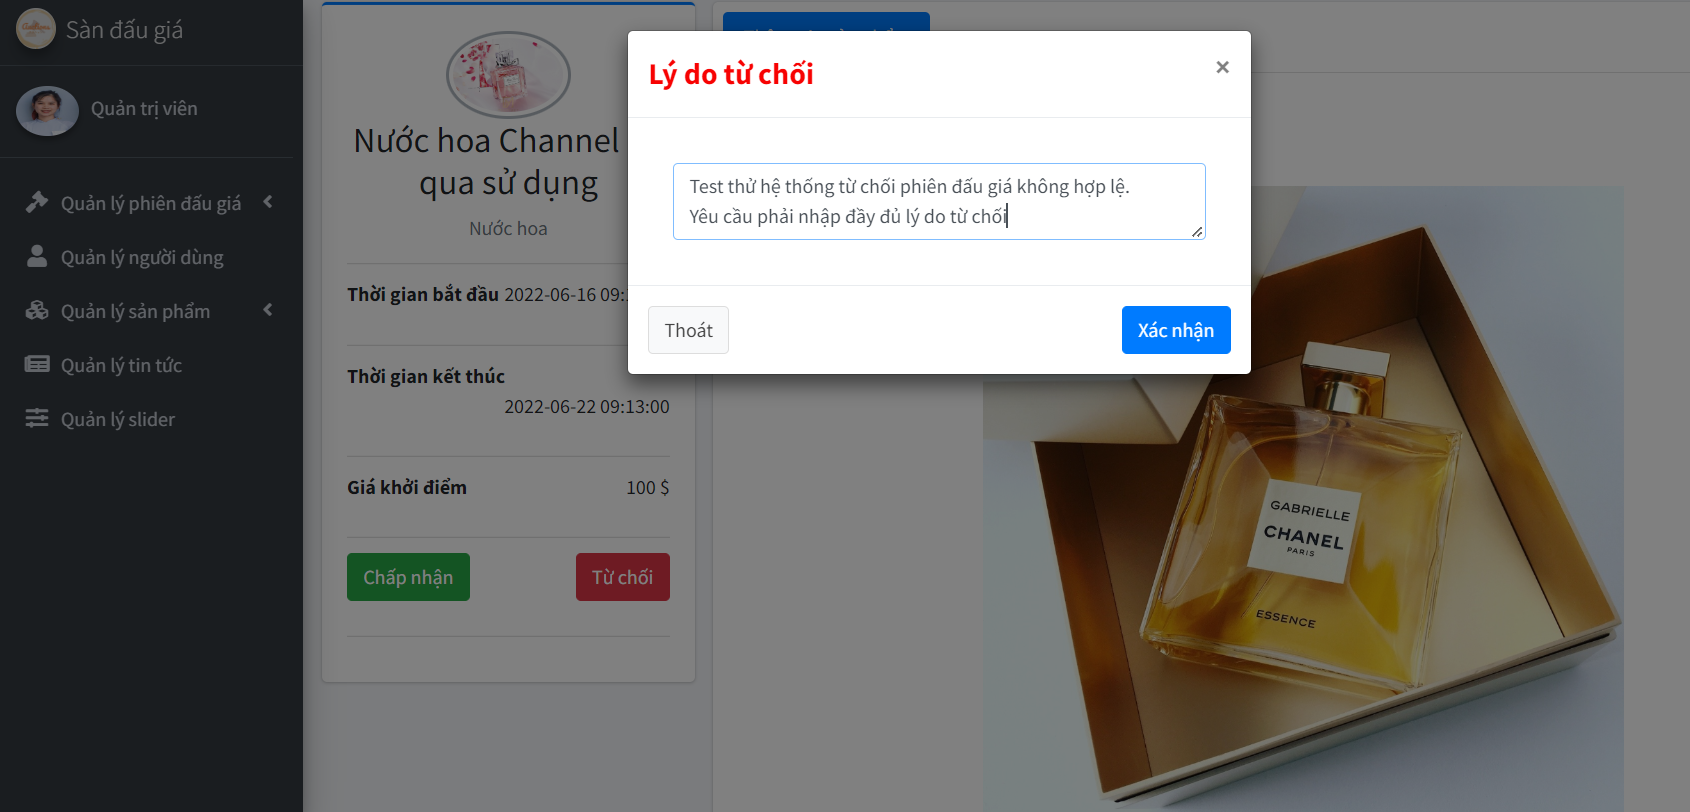
\includegraphics[width=11.4cm,height=4.83cm]{Hinhve/adminreject.png}
\end{figure}
\section{Hệ thống hỗ trợ người dùng có thể tìm kiếm phiên đấu giá theo nhiều tiêu chí}
\subsection{Đặt vấn đề}
Khi hệ thống có nhiều dữ liệu hơn thì việc tìm kiếm một phiên đấu giá phù hợp với nhu cầu của người dùng là mất rất nhiều thời gian. Thay vì người dùng phải lướt từ trên xuống dưới, vào xem chi tiết từng phiên đấu giá để tìm kiếm phiên đấu giá phù hợp với mình thì chức năng tìm kiếm là một giải pháp hữu ích.
\subsection{Giải pháp và kết quả đạt được}
Để giải quyết vấn đề trên thì em có tham khảo một số sàn đấu giá phổ biến hiện nay, xem cách tìm kiếm phiên đấu giá của các website đó được tổ chức như thế nào. Bên cạnh đó để hệ thống phù hợp với người dùng nhất thì em có tham khảo một số ý kiến người dùng về việc khi tìm kiếm thì người ta quan tâm đến gì nhất, thì hầu hết đều tập trung vào tên phiên đấu giá, thời gian bắt đầu, thời gian kết thúc và giá khởi điểm. 

Áp dụng vào website đấu giá trực tuyến, nhằm vừa giảm thiểu số dữ liệu mà hệ thống phải duyệt qua để tìm kiếm và trả về thông tin mà người dùng quan tâm thì em lựa chọn sẽ tìm kiếm phiên đấu giá theo từng trạng thái và nhóm từ khóa mà người quan tâm như giá khởi điểm, thời gian diễn ra, thời gian kết thúc, tên của phiên đấu giá. 

Dưới đây là một số hình ảnh, kết quả của việc tìm kiếm.

Hình ảnh kết quả tìm kiếm theo thời gian bắt đầu.
\begin{figure}[H]
    \centering
    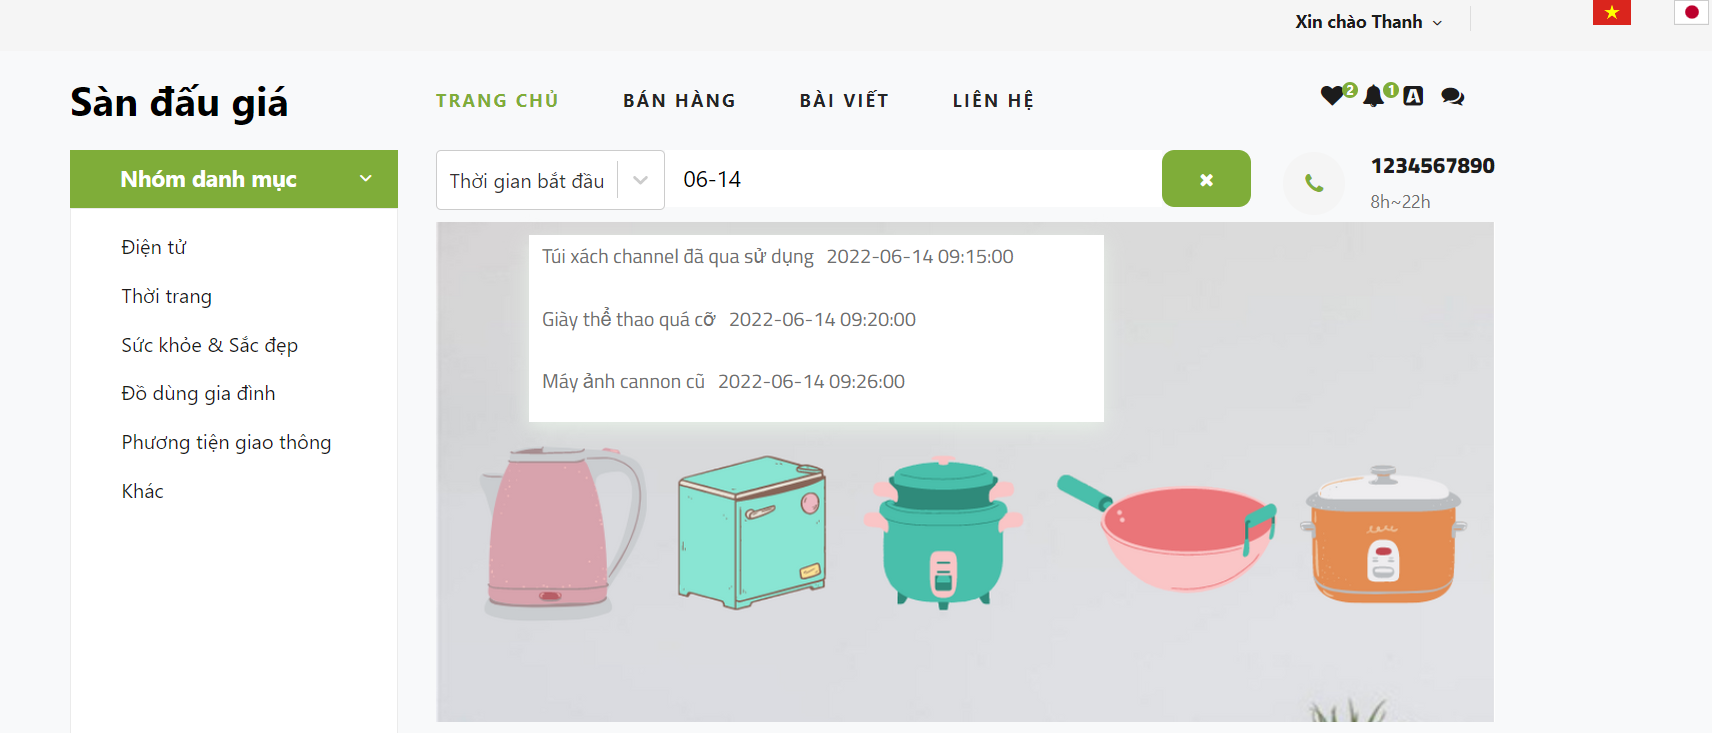
\includegraphics[width=11.4cm,height=4.89cm]{Hinhve/searchstartime.png}
\end{figure}
Ở đây người dùng muốn tìm phiên đấu giá nào có thời gian bắt đầu vào ngày 14 tháng 6. Khi đó hệ thống sẽ hiển thị tên phiên đấu giá và thời gian liên quan mà người dùng tìm kiếm. Nếu kết quả tìm kiếm nhiều thì trên màn hình chỉ hiển thị tối đa 3 phiên đấu giá theo thứ tự thời gian tăng dần, người dùng có thể dùng chuột kéo xuống dưới để thấy các kết quả khác. 

Hình ảnh tìm kiếm phiên đấu giá theo giá khởi điểm.
\begin{figure}[H]
    \centering
    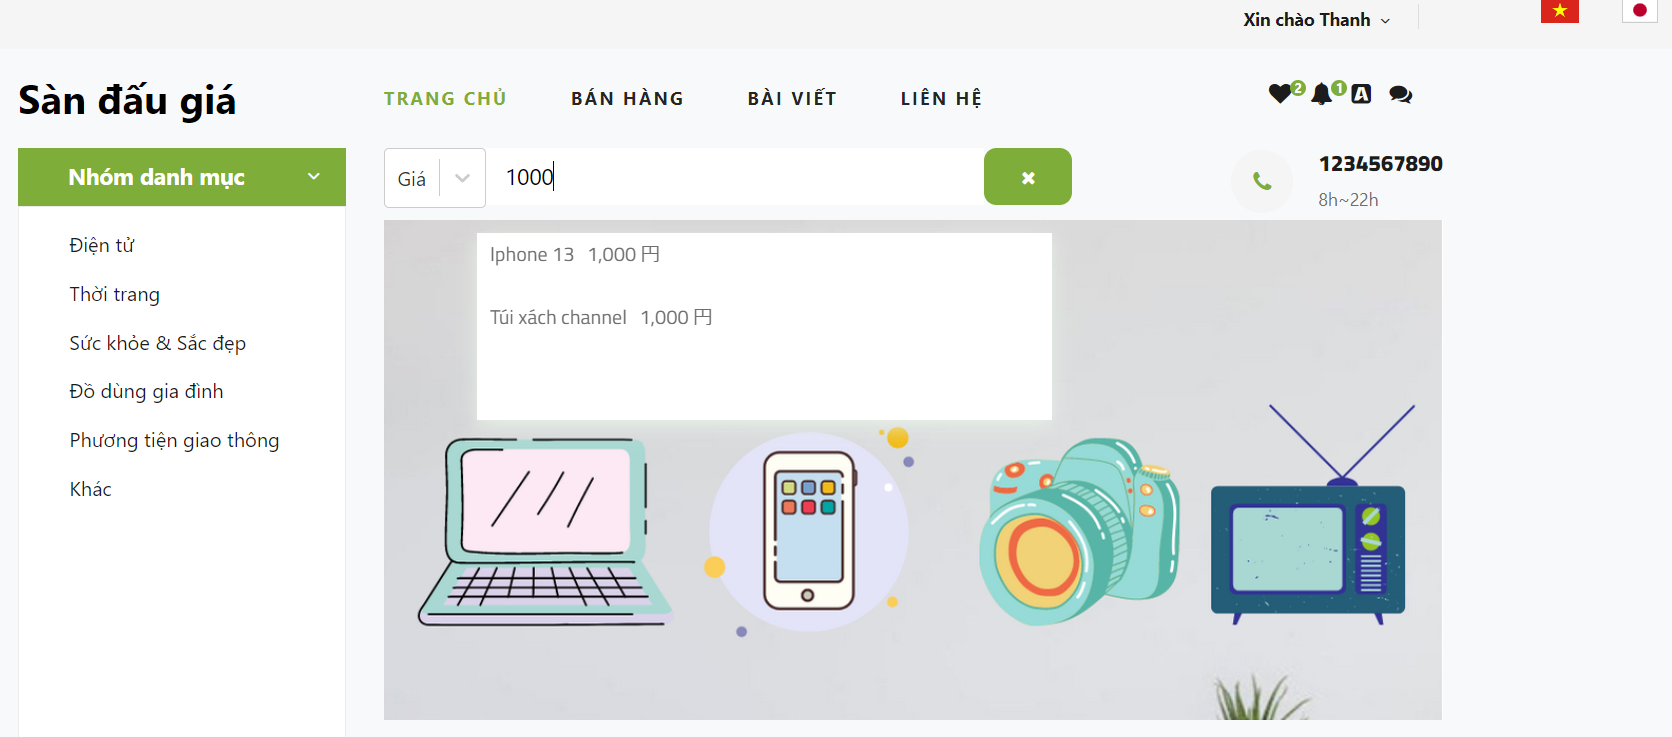
\includegraphics[width=11.4cm,height=4.82cm]{Hinhve/searchprice.png}
\end{figure}
Hình trên tìm kiếm phiên đấu giá theo giá khởi điểm là 1000\$. Hệ thống trả ra kết quả tìm được bao gồm tên phiên đấu giá và giá khởi điểm.
Ngoài việc tìm kiếm trên toàn hệ thống theo từng nhóm từ khóa, thì ở các danh sách phiên đấu giá đã được chia theo nhóm trạng thái thì cũng có thanh tìm kiếm theo tên, theo thời gian bắt đầu, kết thúc của phiên đấu giá. 
\begin{figure}[H]
    \centering
    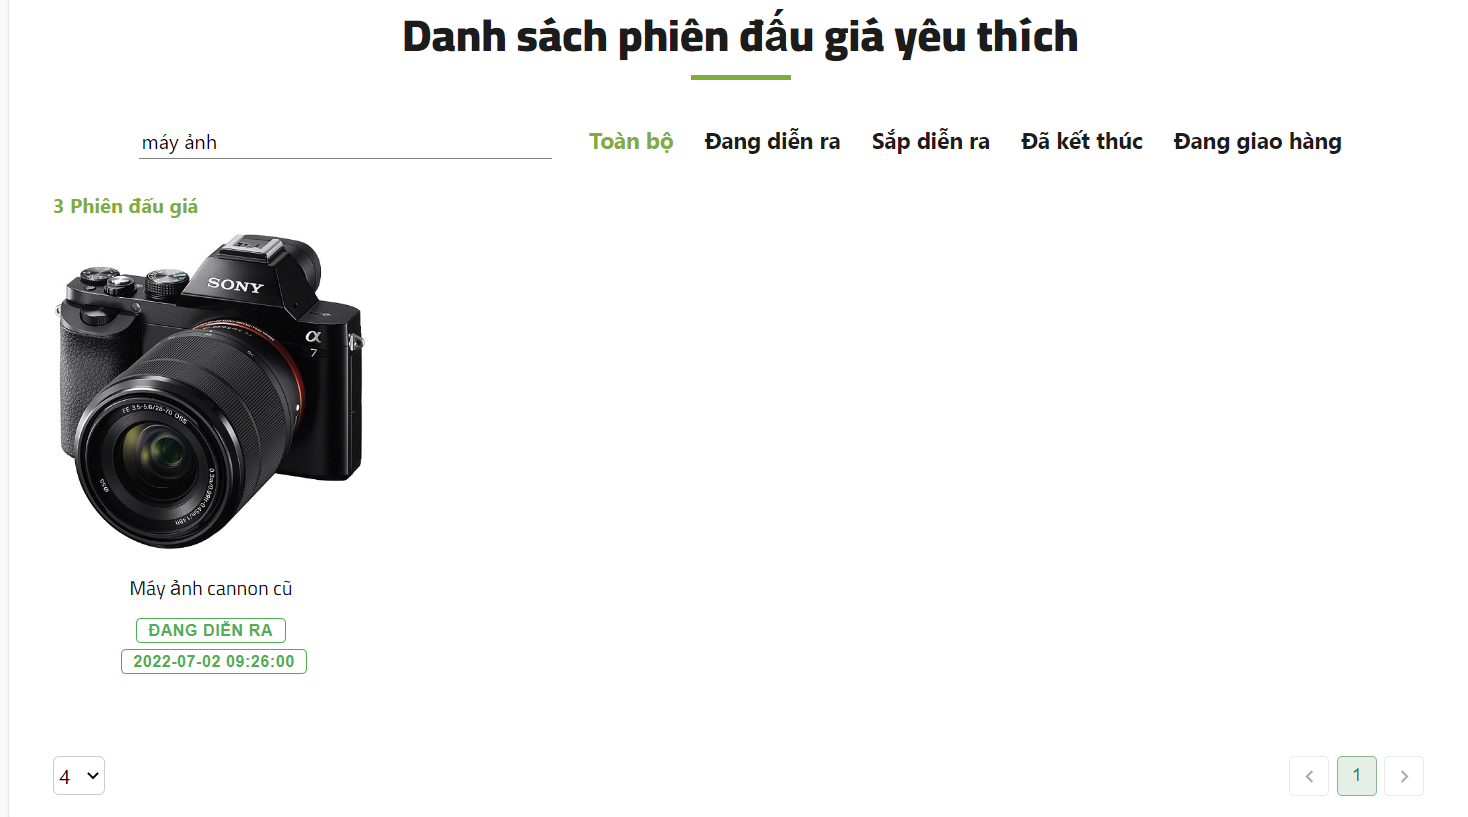
\includegraphics[width=11.4cm,height=6.36cm]{Hinhve/searchlike.png}
\end{figure}
Hình ảnh tìm kiếm phiên đấu giá tại danh sách phiên đấu giá được yêu thích (tại các danh sách phiên đấu giá khác cũng tìm kiếm tương tự)
\section{Hệ thống hỗ trợ nhắn tin trực tuyến}
\subsection{Đặt vấn đề}
Trong quá trình người dùng tham gia đấu giá hay lúc tạo phiên đấu giá, thì vấn đề thắc mắc diễn ra khá thường xuyên.  Nếu chỉ gửi email đợi phía Quản trị viên trả lời thì mất rất nhiều thời gian và khả năng bị trôi email là rất cao; hoặc bình luận trên phiên đấu giá thì cuộc hội thoại không được liền mạch và rất khó nắm bắt nội dung, vì có rất nhiều người bình luận cùng một lúc khiến nội dung bình luận bị trôi. Vì vậy để thuận tiện cho việc trao đổi thông tin, thắc mắc về phiên đấu giá với Quản trị viên, người dùng khác thì một ứng dụng nhắn tin trực tuyến là vô cùng cần thiết. 
\subsection{Giải pháp và kết quả đạt được}
Để giải quyết vấn đề trên thì em có tham khảo các sàn đấu giá hiện nay thì có một số sàn liên kết với các ứng dụng nhắn tin phổ biến như Zalo, Line,.. để liên lạc. Tuy nhiên hiện tại chỉ có người dùng liên lạc với Quản trị viên. Để giải quyết thêm vấn đề có thể trao đổi, liên lạc với các người dùng khác trong website thì em đã quyết định xây dựng một ứng dụng chat sử dụng Socket.IO để đảm bảo tính realtime cho ứng dụng.

Sau đây là một số hình ảnh nhắn tin trên ứng dụng giữa người dùng với người dùng, giữa người dùng với quản trị viên. 

Hình ảnh nhắn tin trực tuyến giữa hai người dùng
\begin{figure}[H]
    \centering
    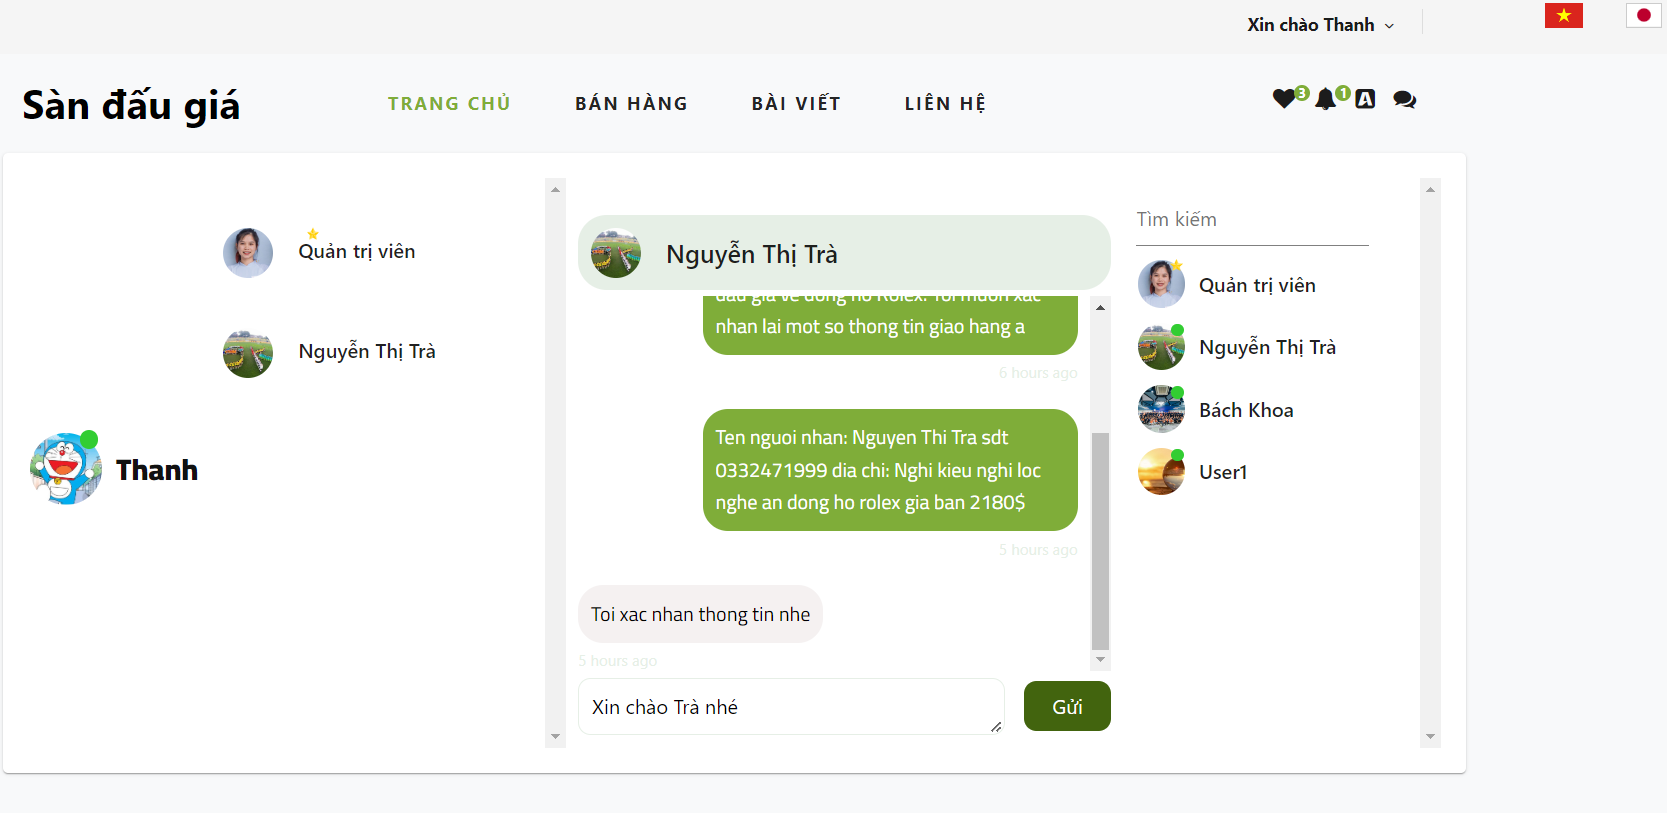
\includegraphics[width=11.4cm,height=5.55cm]{Hinhve/chatuser.png}
\end{figure}
Hình ảnh nhắn tin trực tuyến với Quản trị viên
\begin{figure}[H]
    \centering
    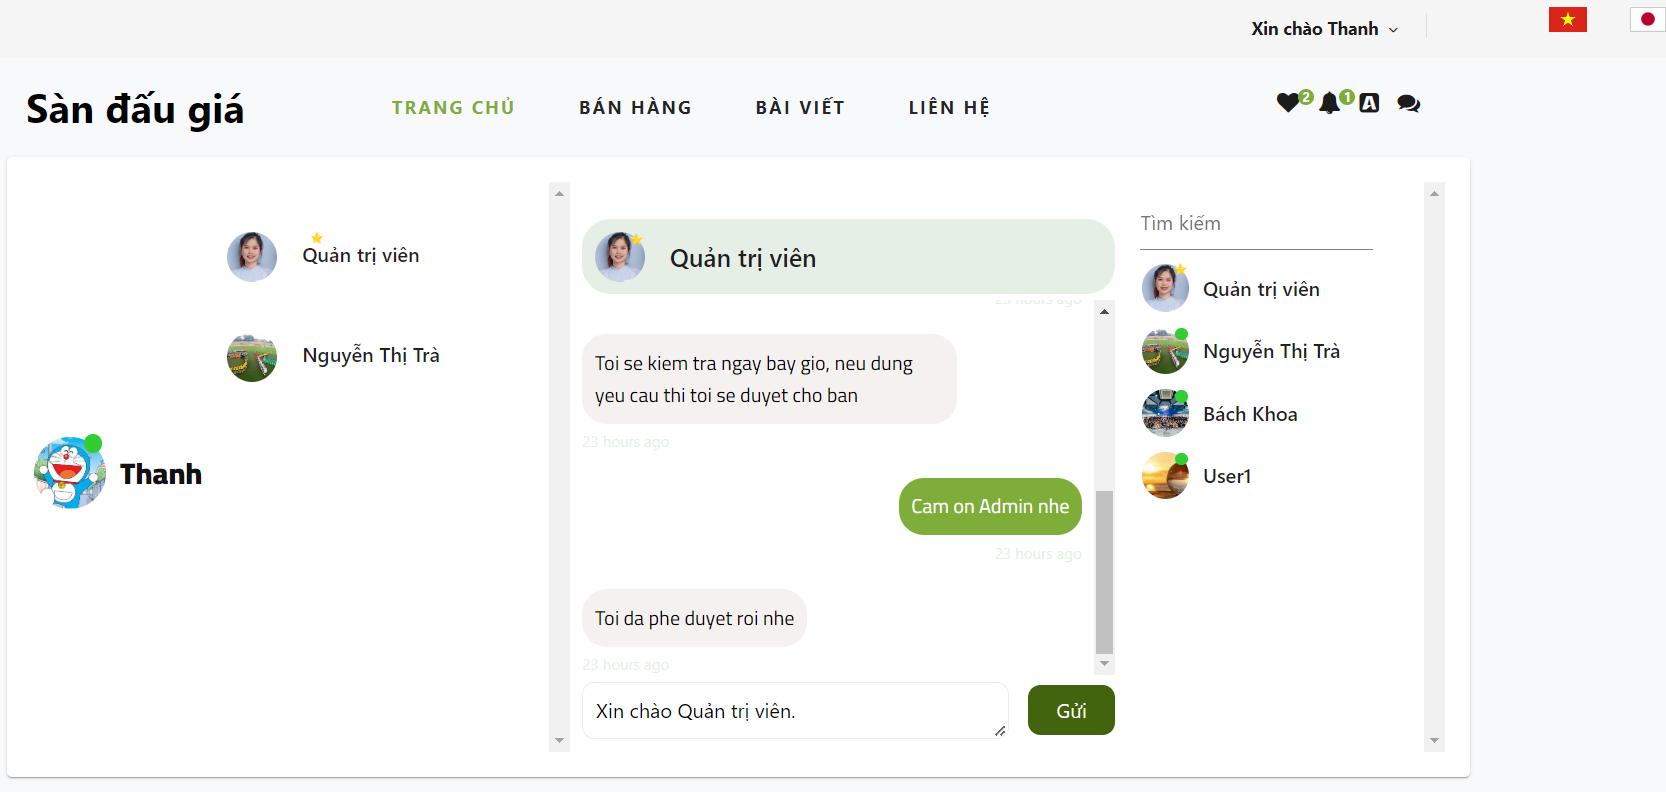
\includegraphics[width=11.4cm,height=5.42cm]{Hinhve/chatadmin.png}
\end{figure}
Để phân biệt giữa Quản trị viên và người dùng bình thường thì với tài khoản Quản trị viên sẽ có ngôi sao ở avatar.
\section{Hệ thống cho phép người mua đánh giá khi nhận hàng}
\subsection{Đặt vấn đề}
Hiện tại thì phiên đấu giá hầu như chỉ diễn ra một lần, sau khi bán sản phẩm đó thì người bán sẽ rất ít khi bán lại sản phẩm đó. Tuy nhiên việc có thêm đánh giá của người đấu giá thành công giúp các người dùng khác nhìn nhận về người bán hàng này một cách khách quan nào đó. Dựa trên đánh giá của người nhận hàng, các người dùng khác có thể nhìn nhận khách quan rằng là người này bán hàng có uy tín không, phiên đấu giá có được thực hiện như quy định không, hay sản phẩm có đúng như mô tả không. Những đánh giá cơ bản đó giúp cho người dùng khác quyết định có nên tham gia phiên đấu giá của người này hay không. Vì vậy việc đánh giá sau khi nhận hàng của phiên đấu giá là rất cần thiết. 
\subsection{Giải pháp và kết quả đạt được}
Giống như các website thương mại điện tử hiện có thì việc đánh giá được thực hiện sau khi người mua nhận được hàng. Đánh giá thì cần có ít nhất 3 yếu tố là nội dung đánh giá, số sao đánh giá và hình ảnh sản phẩm liên quan. Để chắc chắn người mua luôn phải đánh giá sản phẩm thì sau khi người giao hàng xác nhận là đã giao hàng, thì tại giao diện phía người mua sẽ xuất hiện nút xác nhận đã nhận được hàng. Để xác nhận thì người mua bắt buộc phải thực hiện đánh giá, nếu không nhập đủ thông tin thì hệ thống sẽ báo lỗi cho đến khi người mua nhập đủ thông tin hợp lệ. Sau đó đánh giá này sẽ được hiển thị công khai trên phiên đấu giá đó để người dùng khác có thể đọc.

Hình ảnh form đánh giá khi người mua xác nhận đã nhận được hàng.
\begin{figure}[H]
    \centering
    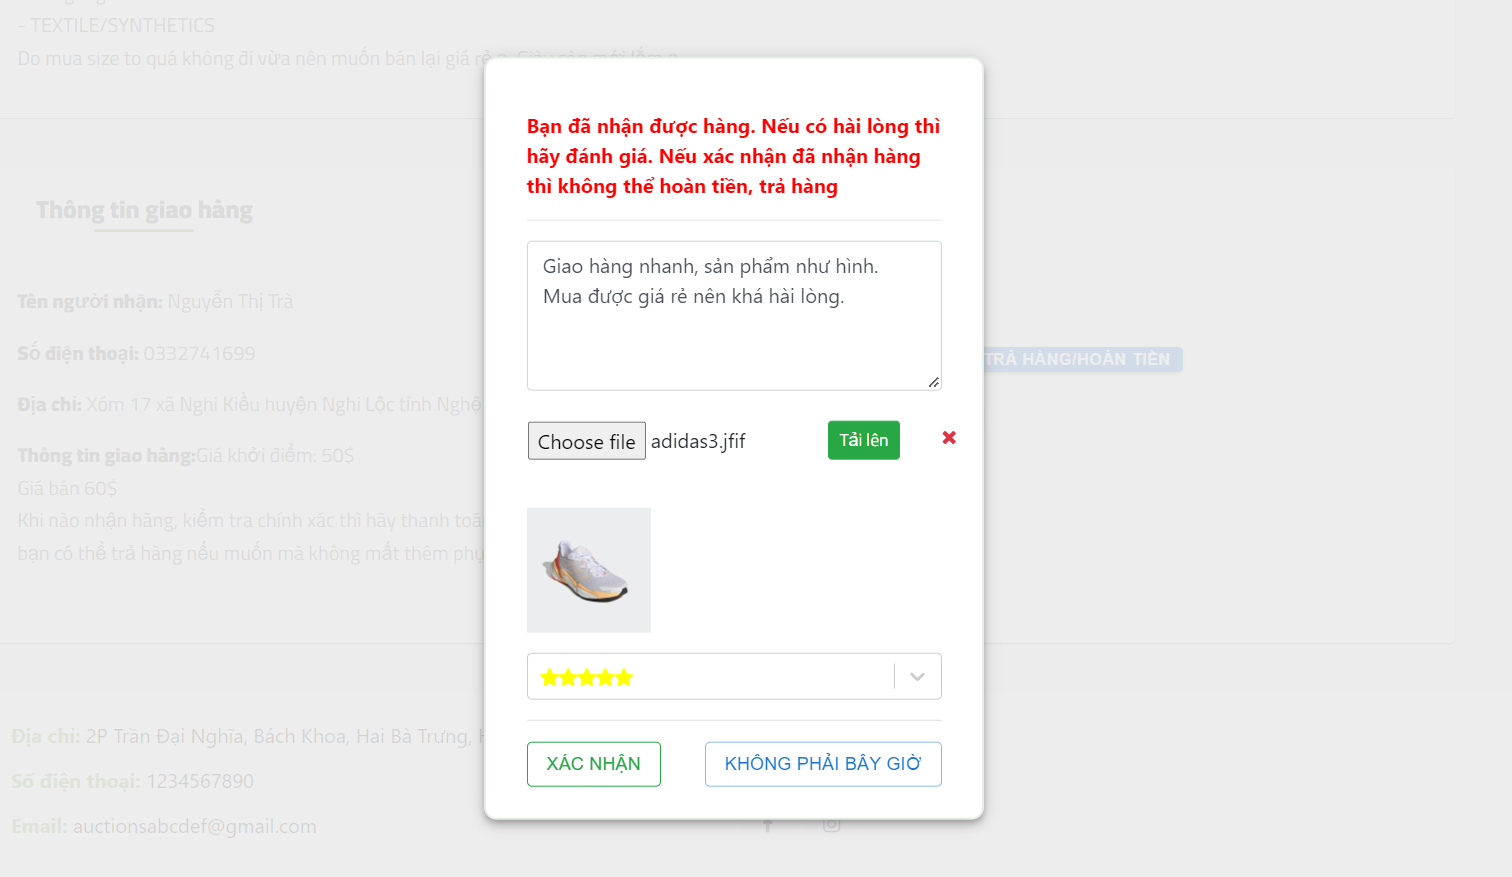
\includegraphics[width=11.4cm,height=6.62cm]{Hinhve/rate.png}
\end{figure}
Hình ảnh đánh giá được công khai lên trên giao diện phiên đấu giá
\begin{figure}[H]
    \centering
    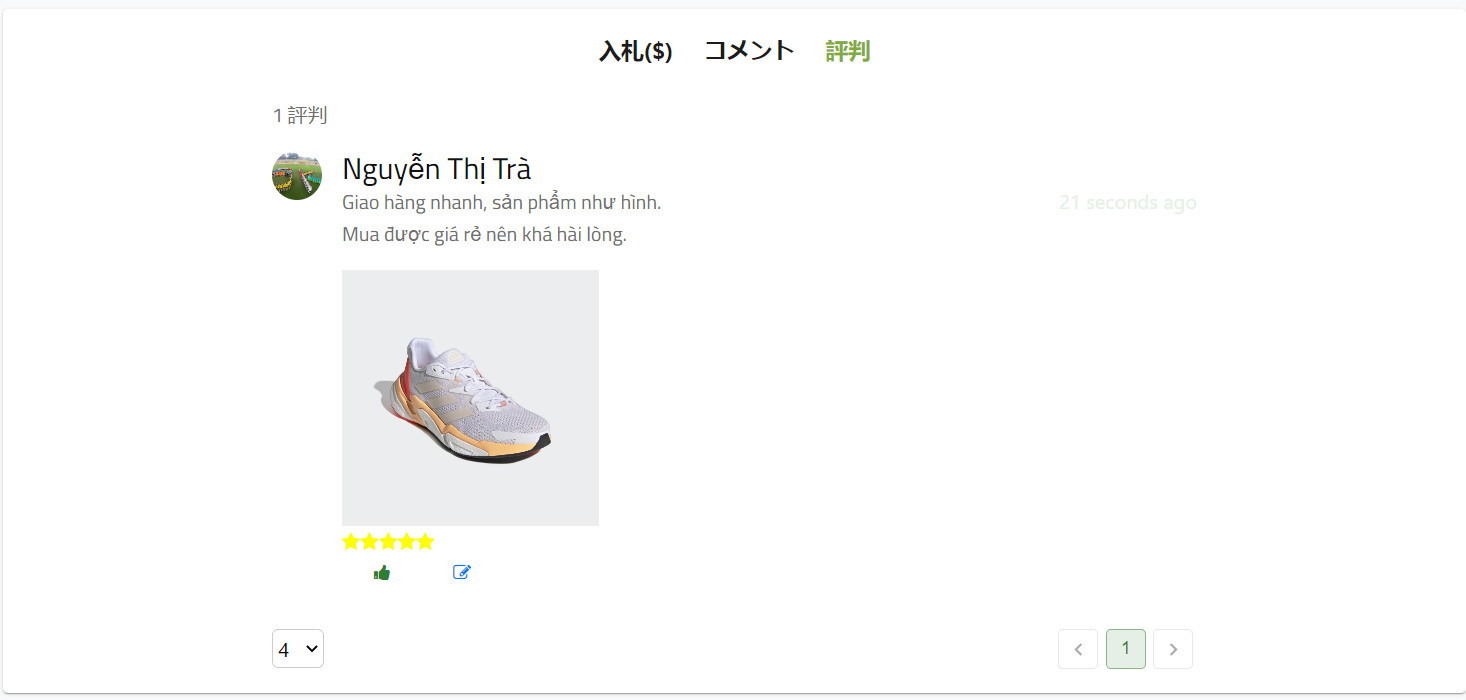
\includegraphics[width=11.4cm,height=5.46cm]{Hinhve/listrate.png}
\end{figure}
\newpage
\end{document}